
\documentclass[letterpaper,hide notes,xcolor={table,svgnames},pdftex]{beamer}
\def\showexamples{t}


%\usepackage[svgnames]{xcolor}

%% Demo talk
%\documentclass[letterpaper,notes=show]{beamer}

\usecolortheme{crane}%seahorse crane
\setbeamertemplate{navigation symbols}{}

\usetheme{MyPittsburgh}
%\usetheme{Frankfurt}

%\usepackage{tipa}

\usepackage{hyperref}
\usepackage{graphicx,xspace}
\usepackage[normalem]{ulem}

\newcommand\SF[1]{$\bigstar$\footnote{SF: #1}}

\usepackage{paratype}
\renewcommand*\familydefault{\sfdefault} %% Only if the base font of the document is to be sans serif
\usepackage[zerostyle=c]{newtxtt}
\usepackage[T1]{fontenc}

\newcounter{tmpnumSlide}
\newcounter{tmpnumNote}

\usepackage{xcolor}
\usepackage{tabu}
\definecolor{light-gray}{gray}{0.75}
\taburulecolor{light-gray}

% old question code
%\newcommand\question[1]{{$\bigstar$ \small \onlySlide{2}{#1}}}
% \newcommand\nquestion[1]{\ifdefined \presentationonly \textcircled{?} \fi \note{\par{\Large \textbf{?}} #1}}
% \newcommand\nanswer[1]{\note{\par{\Large \textbf{A}} #1}}


 \newcommand\mnote[1]{%
   \addtocounter{tmpnumSlide}{1}
   \ifdefined\showcues {~\tiny\fbox{\arabic{tmpnumSlide}}}\fi
   \note{\setlength{\parskip}{1ex}\addtocounter{tmpnumNote}{1}\textbf{\Large \arabic{tmpnumNote}:} {#1\par}}}

\newcommand\mmnote[1]{\note{\setlength{\parskip}{1ex}#1\par}}

%\newcommand\mnote[2][]{\ifdefined\handoutwithnotes {~\tiny\fbox{#1}}\fi
% \note{\setlength{\parskip}{1ex}\textbf{\Large #1:} #2\par}}

%\newcommand\mnote[2][]{{\tiny\fbox{#1}} \note{\setlength{\parskip}{1ex}\textbf{\Large #1:} #2\par}}

\newcommand\mquestion[2]{{~\color{red}\fbox{?}}\note{\setlength{\parskip}{1ex}\par{\Large \textbf{?}} #1} \note{\setlength{\parskip}{1ex}\par{\Large \textbf{A}} #2\par}\ifdefined \presentationonly \pause \fi}

\newcommand\blackboard[1]{%
\ifdefined   \showblackboard
  {#1}
  \else {\begin{center} \fbox{\colorbox{blue!30}{%
         \begin{minipage}{.95\linewidth}%
           \hspace{\stretch{1}} Some space intentionally left blank; done at the blackboard.%
         \end{minipage}}}\end{center}}%
         \fi%
}



%\newcommand\q{\tikz \node[thick,color=black,shape=circle]{?};}
%\newcommand\q{\ifdefined \presentationonly \textcircled{?} \fi}

\usepackage{listings}
\lstset{%
  keywordstyle=\bfseries,
  aboveskip=15pt,
  belowskip=15pt,
  captionpos=b,
  identifierstyle=\ttfamily,
  escapeinside={(*@}{@*)},
  stringstyle=\ttfamiliy,
  frame=lines,
  numbers=left, basicstyle=\scriptsize, numberstyle=\tiny, stepnumber=0, numbersep=2pt}

\usepackage{siunitx}
\newcommand\sius[1]{\num[group-separator = {,}]{#1}\si{\micro\second}}
\newcommand\sims[1]{\num[group-separator = {,}]{#1}\si{\milli\second}}
\newcommand\sins[1]{\num[group-separator = {,}]{#1}\si{\nano\second}}
\sisetup{group-separator = {,}, group-digits = true}

%% -------------------- tikz --------------------
\usepackage{tikz}
\usetikzlibrary{positioning}
\usetikzlibrary{arrows,backgrounds,automata,decorations.shapes,decorations.pathmorphing,decorations.markings,decorations.text}

\tikzstyle{place}=[circle,draw=blue!50,fill=blue!20,thick, inner sep=0pt,minimum size=6mm]
\tikzstyle{transition}=[rectangle,draw=black!50,fill=black!20,thick, inner sep=0pt,minimum size=4mm]

\tikzstyle{block}=[rectangle,draw=black, thick, inner sep=5pt]
\tikzstyle{bullet}=[circle,draw=black, fill=black, thin, inner sep=2pt]

\tikzstyle{pre}=[<-,shorten <=1pt,>=stealth',semithick]
\tikzstyle{post}=[->,shorten >=1pt,>=stealth',semithick]
\tikzstyle{bi}=[<->,shorten >=1pt,shorten <=1pt, >=stealth',semithick]

\tikzstyle{mut}=[-,>=stealth',semithick]

\tikzstyle{treereset}=[dashed,->, shorten >=1pt,>=stealth',thin]

\usepackage{ifmtarg}
\usepackage{xifthen}
\makeatletter
% new counter to now which frame it is within the sequence
\newcounter{multiframecounter}
% initialize buffer for previously used frame title
\gdef\lastframetitle{\textit{undefined}}
% new environment for a multi-frame
\newenvironment{multiframe}[1][]{%
\ifthenelse{\isempty{#1}}{%
% if no frame title was set via optional parameter,
% only increase sequence counter by 1
\addtocounter{multiframecounter}{1}%
}{%
% new frame title has been provided, thus
% reset sequence counter to 1 and buffer frame title for later use
\setcounter{multiframecounter}{1}%
\gdef\lastframetitle{#1}%
}%
% start conventional frame environment and
% automatically set frame title followed by sequence counter
\begin{frame}%
\frametitle{\lastframetitle~{\normalfont(\arabic{multiframecounter})}}%
}{%
\end{frame}%
}
\makeatother

\makeatletter
\newdimen\tu@tmpa%
\newdimen\ydiffl%
\newdimen\xdiffl%
\newcommand\ydiff[2]{%
    \coordinate (tmpnamea) at (#1);%
    \coordinate (tmpnameb) at (#2);%
    \pgfextracty{\tu@tmpa}{\pgfpointanchor{tmpnamea}{center}}%
    \pgfextracty{\ydiffl}{\pgfpointanchor{tmpnameb}{center}}%
    \advance\ydiffl by -\tu@tmpa%
}
\newcommand\xdiff[2]{%
    \coordinate (tmpnamea) at (#1);%
    \coordinate (tmpnameb) at (#2);%
    \pgfextractx{\tu@tmpa}{\pgfpointanchor{tmpnamea}{center}}%
    \pgfextractx{\xdiffl}{\pgfpointanchor{tmpnameb}{center}}%
    \advance\xdiffl by -\tu@tmpa%
}
\makeatother
\newcommand{\copyrightbox}[3][r]{%
\begin{tikzpicture}%
\node[inner sep=0pt,minimum size=2em](ciimage){#2};
\usefont{OT1}{phv}{n}{n}\fontsize{4}{4}\selectfont
\ydiff{ciimage.south}{ciimage.north}
\xdiff{ciimage.west}{ciimage.east}
\ifthenelse{\equal{#1}{r}}{%
\node[inner sep=0pt,right=1ex of ciimage.south east,anchor=north west,rotate=90]%
{\raggedleft\color{black!50}\parbox{\the\ydiffl}{\raggedright{}#3}};%
}{%
\ifthenelse{\equal{#1}{l}}{%
\node[inner sep=0pt,right=1ex of ciimage.south west,anchor=south west,rotate=90]%
{\raggedleft\color{black!50}\parbox{\the\ydiffl}{\raggedright{}#3}};%
}{%
\node[inner sep=0pt,below=1ex of ciimage.south west,anchor=north west]%
{\raggedleft\color{black!50}\parbox{\the\xdiffl}{\raggedright{}#3}};%
}
}
\end{tikzpicture}
}


%% --------------------

%\usepackage[excludeor]{everyhook}
%\PushPreHook{par}{\setbox0=\lastbox\llap{MUH}}\box0}

%\vspace*{\stretch{1}

%\setbox0=\lastbox \llap{\textbullet\enskip}\box0}

\setlength{\parskip}{\fill}

\newcommand\noskips{\setlength{\parskip}{1ex}}
\newcommand\doskips{\setlength{\parskip}{\fill}}

\newcommand\xx{\par\vspace*{\stretch{1}}\par}
\newcommand\xxs{\par\vspace*{2ex}\par}
\newcommand\tuple[1]{\langle #1 \rangle}
\newcommand\code[1]{{\sf \footnotesize #1}}
\newcommand\ex[1]{\uline{Example:} \ifdefined \presentationonly \pause \fi
  \ifdefined\showexamples#1\xspace\else{\uline{\hspace*{2cm}}}\fi}

\newcommand\ceil[1]{\lceil #1 \rceil}


\AtBeginSection[]
{
   \begin{frame}
       \frametitle{Outline}
       \tableofcontents[currentsection]
   \end{frame}
}



\pgfdeclarelayer{edgelayer}
\pgfdeclarelayer{nodelayer}
\pgfsetlayers{edgelayer,nodelayer,main}

\tikzstyle{none}=[inner sep=0pt]
\tikzstyle{rn}=[circle,fill=Red,draw=Black,line width=0.8 pt]
\tikzstyle{gn}=[circle,fill=Lime,draw=Black,line width=0.8 pt]
\tikzstyle{yn}=[circle,fill=Yellow,draw=Black,line width=0.8 pt]
\tikzstyle{empty}=[circle,fill=White,draw=Black]
\tikzstyle{bw} = [rectangle, draw, fill=blue!20, 
    text width=4em, text centered, rounded corners, minimum height=2em]
    
    \newcommand{\CcNote}[1]{% longname
	This work is licensed under the \textit{Creative Commons #1 3.0 License}.%
}
\newcommand{\CcImageBy}[1]{%
	\includegraphics[scale=#1]{creative_commons/cc_by_30.pdf}%
}
\newcommand{\CcImageSa}[1]{%
	\includegraphics[scale=#1]{creative_commons/cc_sa_30.pdf}%
}
\newcommand{\CcImageNc}[1]{%
	\includegraphics[scale=#1]{creative_commons/cc_nc_30.pdf}%
}
\newcommand{\CcGroupBySa}[2]{% zoom, gap
	\CcImageBy{#1}\hspace*{#2}\CcImageNc{#1}\hspace*{#2}\CcImageSa{#1}%
}
\newcommand{\CcLongnameByNcSa}{Attribution-NonCommercial-ShareAlike}


\newenvironment{changemargin}[1]{% 
  \begin{list}{}{% 
    \setlength{\topsep}{0pt}% 
    \setlength{\leftmargin}{#1}% 
    \setlength{\rightmargin}{1em}
    \setlength{\listparindent}{\parindent}% 
    \setlength{\itemindent}{\parindent}% 
    \setlength{\parsep}{\parskip}% 
  }% 
  \item[]}{\end{list}} 




\title{Lecture 22 --- More About Pointers}

\author{J. Zarnett\\
\texttt{jzarnett@uwaterloo.ca}}
\institute{Department of Electrical and Computer Engineering \\
  University of Waterloo}
\date{\today}

\begin{document}

\begin{frame}
  \titlepage
  
  \begin{center}
  \small{Acknowledgments: D.W. Harder, W.D. Bishop}
  \end{center}
\end{frame}


\begin{frame}
\frametitle{Pointers \& Memory Allocation}
First, we examined memory-mapped I/O in which we had agreed upon an address in advance.

When we used a pointer related to a variable, we've just taken the address of an already existing variable (e.g., \texttt{int* ptr = \&y;})

This seems kind of redundant, because we could just use that variable's name, \texttt{y}, instead of using the pointer.

We often want to use pointers to allocate new variables at run-time.\\
\quad The keyword for that in C++ is \texttt{new}.

\end{frame}

\begin{frame}
\frametitle{Run-Time Memory Allocation}
\texttt{int* ptr = new int( 256 );}\\
\quad This allocates memory for a new int and puts the value 256 in it.

Two separate memory locations have been allocated:\\
\quad The integer variable, containing 256; and\\
\quad The pointer \texttt{ptr}, containing the address of the integer.

\begin{center}
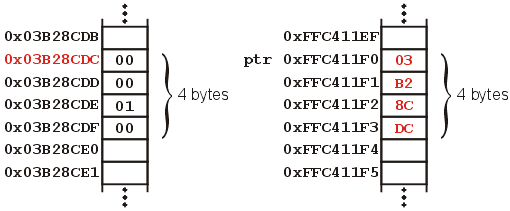
\includegraphics[width=0.75\textwidth]{images/new01.png}\\
{\tiny Image Source: D. W. Harder}
\end{center}

\end{frame}

\begin{frame}
\frametitle{Run-Time Memory Allocation}

When the \texttt{new} keyword was used, the system searched for a block of free memory the size of an integer, and allocated it to our program.

The address of the memory allocated is then stored in \texttt{ptr}.

\texttt{int* ptr = new int( 42 );}\\
A simplified image to picture this statement is:

\begin{center}
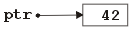
\includegraphics[width=0.2\textwidth]{images/new02.png}\\
{\tiny Image Source: D. W. Harder}
\end{center}

Notice that unlike the usual situation when we allocate an \texttt{int}, there's no variable name associated with the integer variable.

\end{frame}


\begin{frame}
\frametitle{Memory Leaks}

We have already discussed the concept of memory leaks: an area of memory remains allocated even though it is no longer needed.

This happens if we allocate memory with \texttt{new} but forget to tell the system we are done with it when we are finished.

Here is some code that demonstrates how this might happen:\\
\texttt{
\quad int* ptr = new int( 42 );\\
\quad ~ptr = new int ( 1024 );
}

\end{frame}


\begin{frame}
\frametitle{Memory Leaks}
What happened to the memory allocated by the first call to \texttt{new}?\\
\quad It's still there, still contains 42... but we have no way to access it.

We have lost the address of the variable that contains 42 and there's no way to find it again.

\begin{center}
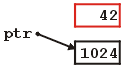
\includegraphics{images/new05.png}\\
{\tiny Image Source: D. W. Harder}
\end{center}

Leaking an integer variable doesn't seem like a big deal given the size of computer memory, but leaks build up over time.

\end{frame}


\begin{frame}
\frametitle{Memory De-Allocation}

Even if we don't reassign \texttt{ptr} and lose the location of a variable, it's still necessary to free up memory when we're finished with it.

The keyword for freeing up that memory is \texttt{delete}.\\
\quad Syntax: \texttt{delete ptr;}

Important: anywhere that \texttt{new} is used on a pointer requires a matching \texttt{delete}, otherwise we leak memory.

After use of \texttt{delete} on a pointer, remember to set that pointer to zero:\\
\quad \texttt{ ptr = 0; }

\begin{center}
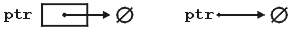
\includegraphics[width=0.5\textwidth]{images/ptr03.png}\\
{\tiny Image Source: D. W. Harder}
\end{center}


\end{frame}

\begin{frame}
\frametitle{Proper Use of Pointers}
Why set pointers to 0 when \texttt{delete} has been called?

If you dereference a pointer containing the address 0, the operating system terminates the program with an error:\\
\quad In UNIX/Mac OS: ``Segmentation Fault (Core Dumped)'';\\
\quad In Windows: You get the ``report problem to Microsoft'' dialog.

Thus, an attempt to dereference the pointer after it's been deleted will result in an error and you will know immediately what went wrong.



\end{frame}

\begin{frame}
\frametitle{Forgetting to Set the Pointer to 0}
If you don't set the pointer to 0, it still contains the old address.

You have called \texttt{delete} so the memory is considered ``free'' and could potentially be allocated for some other purpose.

If you dereference this pointer, several things could happen:
\begin{itemize}
	\item The memory is still there and you can still access it
	\item The memory may be re-allocated to another variable (so two pointers are pointing to the same thing, unexpectedly)
	\item The memory might be allocated to another program; an attempt to access it results in the OS terminating the program.
\end{itemize}

\end{frame}


\begin{frame}
\frametitle{Forgetting to Set the Pointer to 0}
Which of those three outcomes happens is totally random.

Murphy's Law says that the first one will happen in testing; one of the other two will take place when you release the software.

An error that happens only some of the time is much harder to identify and fix than a consistently-occurring error.

If the pointer is set to 0 after \texttt{delete} has been called, the outcome is consistent and we will be able to identify the error straight away.

\end{frame}

\begin{frame}[fragile]
\frametitle{Double \texttt{delete}}

What if we did this?

\begin{verbatim}
int * ptr = new int( 42 );
delete ptr;
delete ptr;
\end{verbatim}

This has the potential to very seriously confuse the system since we marked the memory as free twice.

The system keeps track of what memory is allocated and what is free;\\
\quad Deleting the same location twice corrupts this bookkeeping data.

\end{frame}

\begin{frame}
\frametitle{Double \texttt{delete}}
What happens if we have corrupted the bookkeeping data about what memory is allocated and what is free?

The real answer is ``undefined behaviour'': \\
\quad We cannot predict what will happen.

If you are extremely fortunate it will have no impact.

If you are ``lucky'' the program will crash immediately and you will find the error quickly and correct it before any more damage is done.

More likely, you get negative consequences like silent data corruption.

\end{frame}

\begin{frame}
\frametitle{The Power of Pointers}
Because pointers give developers direct access to memory, they are very powerful tools.

Given a pointer to something on the program stack, it is possible to search for something nearby on the program stack.

The stack is, after all, just a designated area of memory.\\
\quad Given an address in there, we could use pointers to look around.


\end{frame}

\begin{frame}[fragile]
\frametitle{Stack Hack Example}
{\scriptsize
\begin{verbatim}
int enter_number( )
{
    int result;
    cout << "Enter a number: ";
    cin >> result;
    cout << "Address of result on stack: << (int) &result << endl;
    hack_it();
    return( result );
}

int main( )
{
    int i = enter_number( );
    cout << "hack_it( ) already knew you entered << + i << endl;
}
\end{verbatim}
}

\end{frame}

\begin{frame}[fragile]
\frametitle{Stack Hack Example}
{\scriptsize
\begin{verbatim}
void hack_it( )
{
    int x = 0;
    int* a = &x;

    cout << "Address of x on stack: " << (int)&x << endl;
    for( int i = 0; i < 6; i++ )
    {
        cout << a[i] << endl;	
    }
    cout << "You entered " << a[3] << endl;
    }
\end{verbatim}
}

\texttt{hack\_it( )} looks around the stack and knows where to find the number entered.

\end{frame}

\begin{frame}
\frametitle{Comments on the Stack Hack Example}

This example illustrates clearly why passwords stored as plaintext are vulnerable.

If several users were logged in at one time, it might be possible for one user to read confidential data of another.

\end{frame}




\begin{frame}[fragile]
\frametitle{Pointer Arithmetic}

We can use pointers to allocate an array:

\begin{verbatim}
int * array = new int[10];
int* iterator = array;

for( int i = 0; i < 10; ++i) {
    *iterator = 0;
    iterator++;
}


\end{verbatim}


\end{frame}

\begin{frame}
\frametitle{Pointer Arithmetic}

There is did something tricky called \alert{pointer arithmetic}.\\
\quad \texttt{iterator++}

Pointer arithmetic is arithmetic expressions involving pointers.\\
\quad \texttt{(ptr + 1)} adjusts the address stored in the pointer.

Pointer arithmetic works based on the size of the pointer.

If an integer takes up 4 bytes in memory, then {(iterator + 1)} increments the address by 4 (because 4 is the size of an integer).

It allows us to walk through the array without use of the index operator \texttt{[]}.

\end{frame}



\begin{frame}
\frametitle{A Note About C}

C++ is backwards compatible with the C programming language, so C syntax is valid in C++.

When allocating memory in C++, the \texttt{new} keyword figures out the correct amount of memory for our request. E.g. the size of an \texttt{int}.

In C the routine to allocate memory is a function \texttt{malloc( )}.

This function takes one parameter: the size of memory requested.

\end{frame}



\begin{frame}
\frametitle{Use of \texttt{malloc}}

If we know that an integer is 4 bytes, we may simply call \texttt{malloc()} with the parameter 4.

This is, however, bad practice. For compatibility and portability reasons, there is an additional operator to find the size of the type.

This is the \texttt{sizeof} operator, and it takes a type as its parameter.

\texttt{ int *x = malloc( sizeof( int ) );}\\
\quad Will allocate the correct amount of memory for an integer.

The \texttt{sizeof} operator can also be used on programmer defined types.

\end{frame}



\begin{frame}
\frametitle{Use of \texttt{malloc}}

For an array of capacity 10:\\
\quad \texttt{int *array = malloc( 10 * sizeof ( int ) );}

So a memory array is just a pointer. And we use the capacity of the array as a multiplier times the size of the type.

\end{frame}



\begin{frame}
\frametitle{Deallocation}

Deallocation works similar to the \texttt{delete} keyword.

The function for deallocation is \texttt{free( )} and it takes a pointer.

Example: \texttt{free( array )}.

Just as with \texttt{new} and \texttt{delete}, every call to \texttt{malloc( )} must be matched to a call to \texttt{free( )}, otherwise memory is leaked!


\end{frame}

\end{document}

